\twocolumn[
\centering
\LARGE Appendix 2: ELEN4002 Project Plan
\linebreak
\normalsize Darrion Singh (1056673) and Sachin Govender (1036148) -- Group 35
\linebreak
]
\begin{abstract}
This report contains a project plan to implement an image-based digital Body Mass Index (BMI) estimator.
The estimator is to be a robust and accurate alternative BMI estimation to the classical height and mass measurement.
The major benefit of the estimator is the neccessary ability to assess large groups of people in a relatively quick manner.
Literature related to image processing and neural networks were consulted to propose a system to accurately estimate BMI.
The proposed solution consists of taking a front and side view image of participants and using feature extraction methods such as Object Detection and Image Segmentation to obtain various measurements across the body.
Thereafter the measurements should be passed into two independent neural networks that estimate BMI based on front view data, separately from side view data.
These two independent BMI estimates are passed through a neural network that provides an averaged weighting to obtain a final BMI estimate.
In order to create the proposed system, a data-set of photographs, mass, height, and optionally race and sex will be obtained from research clinics in order to train and test the models in the system.
Image processing and machine learning will be carried out in Python with the aid of the OpenCV, Tensorflow and Keras libraries.
The project is expected to be concluded within six weeks and must aim to meet the success criteria of having a maximum of 2\% error.
Difficulties are expected in the form of time limitations, data-set inadequacy and potential over-fitting.
These issues can be mitigated through extending the data collection time, increasing the size of the data-set and ensuring a relatively equal distribution of participants in terms of age, race and gender. 
\end{abstract}
\section{Introduction} \label{intro}
The Body Mass Index (BMI) is a metric used as an indication of whether one's body mass is healthy for their corresponding height \cite{nhsBMI}.
Whilst not an accurate diagnostic tool, the BMI provides a healthy body mass range for a particular height as it takes into account natural body shape variations \cite{nhsBMI}.
Unfortunately, the accurate collection of ones height and mass is time-consuming, especially when considering the time required to collect this data for large amounts of people.
This project investigates the potential for a digital estimation of one's BMI from a photograph, using a mixture of Computer Vision and Machine Learning.
The following report contains the proposed methods and respective schedules associated with the undertaking of this project.

\section{Background}
\subsection{Project Concept}
The aim of this project is to estimate, to a reasonable degree of accuracy, the BMI of a person from their photograph.
This is to be achieved by the creation of a program which accepts a photograph of a person, extracts body shape data from the photograph and with the use of a machine learning algorithm, predict one's BMI based on their body shape data.
The purpose of such a tool has vast applications in the medical field, whether it be used as a time-efficient means of tracking the progress of a disease/disorder that increases/decreases ones mass, or for a simple indication of ones own health.

The success of this project would result in the production of a mobile BMI estimator which precludes the need for a subject to remove their clothes, saving practitioners time for BMI measurement.
In large rural clinics, where large patient volumes combined with time taken to undress and redress for accurate height and mass measurements, this digital solution may result in a significant reduction in the time taken for consultations.
Furthermore, this solution would not be affected by measurement errors resulting from incorrect calibration.
\subsection{Assumptions \& Constraints}
As to provide the least chance of a false human body outline being detected, we assume that any person being photographed is staged in front of a uniform background, such as a wall of distinct uniform colour.
As such, all photographs used to train the machine learning algorithm should abide by the same assumption.
In order to provide a distance reference, each photograph should contain a shape of known dimensions.
For consistency, the shape should be the same in all pictures, as well as having the same colour and the same dimensions.
This reference object must be present both during training and live testing.
Furthermore, the distance between the camera and the subjects being photographed should remain static and be far enough away to capture the subject's full body photograph, where the subject is a maximum of two meters tall.
The time frame for this project is seven weeks, with a total budget of R1200.
\subsection{Success Criteria}
As this solution means to be time efficient, it aims to negate the need for one to remove their clothes as is usual with regular BMI measurement.
Thus, the program should be able to operate with pictures of people who are clothed.
The estimation should also be possible using pictures of varying resolutions, i.e. the solution must work for multiple cameras.
The specified success criteria error has been given as 2\%, however the upper limit of the BMI is generally given as 40 \cite{nhsBMI}. This translates to an absolute error of 0.8 such that for an actual BMI of 20, an estimated value between 19.2 and 20.8 will be considered as accurate enough.
\subsection{Optional Criteria}
Since the purpose of digital estimation of BMI is the production of a solution that is mobile and not time-consuming, it would be ideal if the software and it's trained neural network models were exported to either a mobile application or desktop executable.
In this way, one could select a photograph from their cellphone/desktop gallery and the program could perform estimation on the chosen picture.

Furthermore, to improve the robustness of the design it would also be most ideal if the application/executable could receive pictures from a connected camera.
In the case of the mobile application, it would access the cellphone's camera and perform a BMI estimation from a photograph taken in-app.
This would potentially expand the use of the machine learning algorithm to be used by the general consumer with minimal effort.

As seen in Ref. \cite{bmiage}, there are significant statistical variations in the BMI of male and females across age groups.
Provided that there is sufficient training data, one final manner of decreasing the effects of sex bias in the data from the photographed subjects would be to train two separate models for male and female data points.
The exclusion of the male data from the female model and visa-versa will improve accuracy by modelling a specific BMI distribution for each sex, as to statistically correlate with Ref. \cite{bmiage}.
\section{Training Data Collection}
\subsection{Data Types}
The data to be collected are as follows:
\begin{itemize}
\item A front and side photograph of the subject.
Both photographs should have the reference object in the top left corner of the image.
As mentioned above, the background of the image should be a uniform surface such as a wall.
This is to ensure that the image pre-processing techniques described in the succeeding sections of this report can be carried out without error.
\item The height and mass of each person.
These must be captured simultaneously and attached to the front and side photographs.
Data survey applications such as \textit{REDCap} may be useful in achieving this.
\item (Optional) Sex of person in each photograph.
Whilst this characteristic is not an input into the system, it should be recorded for statistical purposes for later quantification of algorithmic bias.
Furthermore, to achieve the optional criteria discussed above, data points must be labelled as male/female to train separate models.
\item (Optional) Race of person in each photograph.
This characteristic could also be recorded for statistical purposes.
Furthermore, it opens an avenue for further research into how ethnicity can be used to narrow BMI distribution and hence provide more accurate BMI estimations.
\item (Optional) Age of person in each photograph.
This characteristic, despite only being recorded for statistical purposes, is by far the largest contributor to the distribution of BMI, as seen in Ref. \cite{bmiage}.
Knowing the distribution of the age of the subjects will provide a range of ages where the program is likely to provide the most accurate estimation.
\end{itemize}
With the ultimate aim in mind for this program to be a universal BMI estimator, it is encouraged that the data-set of subjects who volunteer to be photographed be spread in terms of sex, ethnicity and age.
\subsection{Obtaining Data}
It is possible to find such images of people on the internet, however it is unlikely for these images to have the corresponding height and mass on record.
The chosen method for obtaining the data is to illicit the help of a medical research group who have access to large amounts of people, along with properly calibrated height and mass measuring equipment.

It should be noted that obtaining data in this manner requires prior clearance from a recognised ethics committee, as well as the permission of those in charge of the proposed sites such as research clinics.
As with most neural network related projects, it is encouraged for a large data-set to be collected, and it was decided that a reasonable minimum number of subjects would be 100.
\section{Literature Review}
Before deciding on the proposed solution described in the succeeding sections, various academic literature regarding image processing and machine learning were consulted.
The following provides a summary of findings that were considered when deciding upon the final solution.

\subsection{Weight and Diameter Estimation}
Comert et al. aims to estimate the mass of an apple through image processing and machine learning techniques \cite{comert}.
The process involves using the Prewitt edge extraction algorithm in order to obtain a binary image.
The binary image goes through Closing, filtering and Opening.

Closing is the process of performing Dilation followed by Erosion on an image, whilst Opening is the process of performing Erosion followed by Dilation on an image \cite{opening,closing}.
Dilation is a morphological operation whereby the value (intensity) of a pixel is increased to that of the pixel in its neighbourhood with the highest intensity \cite{mathworksdilationerosion}.
Erosion is a morphological operation whereby the value of a pixel is decreased to that of the pixel in its neighbourhood with the lowest intensity \cite{mathworksdilationerosion}.
This is done in order to improve the image quality for feature extraction, since Closing an image improves the prevalence of contours, whilst Opening an image improves the uniformity of the spaces between contours.
Figure \ref{fig:segmentedapples} shows the segmentation stage of the apple image.
\begin{figure}
    \centering
    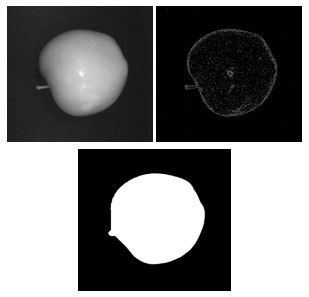
\includegraphics[width=\linewidth]{segmentedapples.jpg}
    \caption{Segmentation techniques to isolate the apple in the image \cite{comert}.}
    \label{fig:segmentedapples}
\end{figure}

Feature extraction is carried out such that the area and diameter of the apple are extracted, thereafter the diameter and the recorded masses are used in a linear regression model.
Figure \ref{fig:diameterapples} shows the diameter extraction from the images.
\begin{figure}
    \centering
    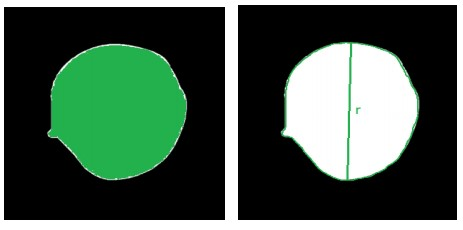
\includegraphics[width=\linewidth]{diameterapples.jpg}
    \caption{Apple Area and Diameter Extraction  \cite{comert}.}
    \label{fig:diameterapples}
\end{figure}
\subsection{Weight Estimation Using Image Analysis and Statistical Modelling}
Similar to the requirements of the BMI system, Kollis et al. discusses a robust image analysis based mass estimation of pigs in large scale livestock farming \cite{kollis2007weight}. 
The software of choice for image processing is MATLAB in which the Image Processing Toolbox V4.1 is used.
Object detection occurred through comparison between the camera environment without the pig and with the pig.
This results in a binary image that undergoes segmentation, filtering and opening to get a clear image for feature extraction.

Feature extraction in this paper is particularly useful as the body shape of the pigs is more complex than the apple described in the previous review. 
The feature extraction method is comprised of the skeletonisation function in MATLAB which generates a skeletal structure of the object in question.
Figure \ref{fig:pigskeleton} shows the skeletonisation process for the image of the pig.
\begin{figure}
    \centering
    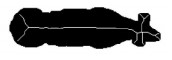
\includegraphics[width=\linewidth]{pigskeleton.jpg}
    \caption{Skeletonisation function implemented on pig binary image\cite{kollis2007weight}.}
    \label{fig:pigskeleton}
\end{figure}

Using this process the spine (main branch) is used to estimate the length of the pig by counting the pixels which comprise the spine.
Thereafter the estimated length and recorded masses were used in a linear regression model to estimate mass.
\subsection{Human Weight from a RGB-D Image}
Nguyen et al. explores human mass prediction through a single RGB-D image \cite{nguyen2014seeing}.
The camera in question uses a depth sensor to create a separate depth image. 
This extra image proves to be useful in object detection due to depth allowing an accurate trace of the human body shape with the aid of the 2D RGB image. 

This method is more accurate than the common rectangular object identification method. 
This silhouette is passed through similar image processing methods used in the aforementioned papers. 
However, mass prediction is different in this scenario as the author used various mathematical relationships relating body width, height and area with Support Vector Regression -- as opposed to machine learning -- to predict the mass of the person through the extracted features. 
\subsection{Types of Neural Networks}
Mehta discusses the various types of neural networks and what applications in which they prove to be useful \cite{mehta_2019}. 
In summary: Feed-Forward neural networks were useful in situations with minimal data-sets, as well as data-sets that have a substantial amount of noise.
The multi-layer perceptron is used when the training data-set is not linearly separable.
Networks that make use of back propagation need large data-sets and is generally used in when the network needs to recall or retain information.
Convolutional neural networks are used in applications such as object detection and image classification.
\section{System Design}
The proposed solution comprises of two subsystems, namely the Extraction layer and the Machine Learning layer.
These subsystems have no dependency on each other and are to be built independently of one another.
Figure \ref{fig:systemblockdiagram} in the Appendix provides a system diagram showing the inputs and outputs of each system, as well as the components of each system.
As seen, the Extraction layer comprises of the Object Detection, Image Segmentation and Input Extraction components.
The Machine Learning layer comprises of the Front View, Side View and Weighted Averaging components.
\subsection{Extraction Layer}
A front and side view photograph of a person with a reference object in the top left corner is the input into the system.
Object Detection will isolate the two objects in the photograph, namely the person and the reference object \cite{objectDetection}.
The dimensions of the bounding box surrounding each object, measured in pixels, will be converted into meters using the known physical dimensions of the reference object.
This is done by computing the meters per pixel metric \cite{objectDetection}.
The vertical dimension of the person's bounding box, i.e. their height, is one of the outputs of the subsystem.

For both the front and side view photographs, each original unprocessed image will undergo Image Segmentation separately.
The Image Segmentation process will locate the pixel mask -- all pixels belonging to an object -- of the two objects in each photograph, although only the masks of the person is required \cite{semantic,instance}.
Using the meters per pixel found in the previous component, different horizontal slices of the person's pixel masks will be extracted as the width (for the front view photograph) and depth (for the side view photograph) of the person at their corresponding heights above the ground.
The final number of width/depth measurements as well as the height at which they will be taken is unknown, and it is only through testing that the optimum number of slices/heights can be determined.
Finally, using the meters per pixel metric, the pixel masks will be converted into a physical two dimensional area.

The output of the Extraction layer will two vectors, namely the front view vector (FVV) and side view vector (SVV).
The FVV will comprise of the person's front view area, and the person's width at various heights.
The SVV will comprise of the person's side view area, and the person's depth at various heights.
It is important to note that the chosen heights for the width/depth measurement \textbf{must} be the same, such that corresponding indices of the FVV and the SVV refer to the same height above the ground.
\subsection{Machine Learning Layer}
All the outputs of the Extraction layer mentioned above are provided as inputs into the Machine Learning layer.
The front view and side view outputs are passed into the Front View and Side View components independently, both of which are neural networks.
Both networks will be trained to estimate BMI independently until an acceptable accuracy is achieved, or falling short of that, the best possible accuracy is achieved.

The estimated BMI from the Front View and Side View component are then used as inputs into a final neural network, the Weighted Averaging component.
This network will be trained to estimate BMI by deciding the contribution that the front and side view images should make to obtain a final BMI estimation with improved accuracy.
\section{Methodology}
The above processes can be done using multiple image processing libraries with languages such as Python, R, MATLAB etc.
However, due to its open-source nature, large online community support, and its growing popularity in the Machine Learning field, this project will be created using Python.
Currently, there is no indication that any other language or software package will be required to implement this project, however, any deviations from this statement will be minimised as far as possible and be documented.
The following section breaks down the methodology employed to achieve each component and subsystem implementation, as well as the potential tools that may be used.
\subsection{Extraction Layer}
\subsubsection{Object Detection}
The ultimate purpose of the Object Detection component is to extract the meters per pixel metric from the photograph, since this metric is used for all subsequent data extraction in the succeeding components such as the person's height, width and depth.
The manner in which this is to be performed, using the OpenCV-Python library, is as follows: The image is first converted to grayscale (commonly referred to as a black and white image), and slightly blur it \cite{objectDetection}.
The purpose of this is to decrease the effects of noise in the picture, which manifests as random sharp changes in the picture such as a scratch on a uniform surface -- a distinct line that does not contribute to the contour of any object.

Closing is then performed on the image to remove any gaps in a border line that might prevent contour detection \cite{objectDetection}.
All contours in the image are then detected and ordered from left to right \cite{objectDetection}.
As mentioned in the previous sections, the reference object must be placed in the top-left corner -- this choice was to facilitate contour detection, and ensuring that the reference contour is always evaluated first.
We then discard false contours detected by OpenCV by setting a minimum contour length \cite{objectDetection}.
This value needs to be sufficiently small to prevent the reference object from being discarded, but large enough that minute details about the person is discarded, such as their eyes and mouth.

The reference object bounding box and person object bounding box is then extracted from the image \cite{objectDetection}.
Using the known dimensions of the reference object, extract the physical vertical dimension of the person object bounding box, and provide it as an output of the Extraction layer.
\subsubsection{Image Segmentation}
The ultimate purpose of the Image Segmentation component is to extract the width and depth of a person from the front and side view photographs respectively, since these two characteristics (at specified heights) are data points for the FVV and SVV respectively.
The manner in which these are extracted, using the OpenCV Python library, is as follows:
Using a trained masking model such as ENet or Mask R-CNN, the images will have instance or semantic segmentation performed on them \cite{semantic, instance}.
Due to the assumption that only one person will exist in the photograph, with the rest of the image in the background, there will only ever be one instance of a person in the image, and as such, either semantic or instance segmentation should be sufficient to extract the mask.

Once the pixel mask has been isolated, the pixels along a certain row (specified height) of the mask will be summed and converted to distance, yielding the width/depth for front/side pictures.
Finally, a simple pixel to area conversion will yield the mask's corresponding physical area after summing the number of pixels in the entire mask.
These widths, depths, and areas will be extracted and provided as outputs of the Extraction layer.
\subsection{Machine Learning Layer}
As per consulting the aforementioned Literature Review, it must be noted that the simplest type of Neural Networks that may account for a noisy, small, and potentially linearly inseparable data-set are the Feed Forward or Artificial Neural Network, and the Multilayered Perceptron.
These network models are relatively simple to implement due to their lack of kernel requirements or back propagation, and as such are conducive to implementation via a well documented medium such as Python.
In particular, libraries such as TensorFlow and its complementary libraries such as Keras are thoroughly documented in the field of Machine Learning.
These libraries will be used to create and train the Front View and Side View component models, as well as the Weighted Averaging component model.

The data-set will be split into 70\% used for training, and 30\% for testing and validation.
Training will halt via the early stopping mechanism, which stops a model from training past a certain metric -- in this case being the Mean Absolute Error \cite{bmifromface}.
This early stopping will prevent over-fitting of data points and thus aims to improve generalisation of the model.

Finally, it is important to note that whilst the Front and Side View models are to be trained with the data from the Extraction layer, the Weighted Averaging layer can only be trained once the Front and Side View models are trained.
This is due to the fact that the Weighted Averaging model training data-set is to be generated from the output of the Front and Side View models.
\section{Project Management}
As stated above, six weeks have been given to deliver a working solution.
Due to time being limited, it is imperative to optimise the productivity of the development of the project through scheduling and resource allocation.

The working hours on the project have been summarised as follows: 
\begin{itemize}
    \item The work weeks consist of the five weekdays.
    \item Working hours lies between 10:30 and 18:00.
    \item Time spent on the project during weekends and times outside of working hours are considered as overtime.
\end{itemize}
	 
The resources available for the project are:
\begin{itemize}
    \item The Primary Investigators.
    \item Supervisors.
    \item Clinic Staff.
    \item Smartphone cameras with a minimum quality of 15 megapixels.
    \item Three Laptop/Desktop computers with a minimum processing speed of 2.5GHz, 8GB of RAM, two of which have GTX-1050 GPUs.
    \item Cloud storage sufficient to store photograph backups.
\end{itemize}

Figure \ref{fig:gantt} in the Appendix provides a Gantt chart that summarises the work breakdown during the course of the project.
The tasks allocated to the primary investigators are as follows: Darrion Singh is allocated the Extraction layer (Image Processing) and Sachin Govender is allocated the Machine Learning layer (Neural Network).
The time allocated to the project is split as shown in Figure \ref{fig:gantt}, however there is a possibility of both investigators facilitating each other on their respective tasks due to unforeseen circumstances such as task difficulty or slack in a parallel task. 
\section{Expected Challenges}
An neural network based model is only as good as the size and quality of the data set used for training.
Due to the limited time available for data collection, there is possibility that the data acquired may not create a model that meets the success criteria.
Excluding time sensitivity, the data acquisition can be further hindered by multiple factors such as clinic facilitators/data collectors not following procedure correctly, resulting in the reduced quality and size of the data-set.
Preventative measures for data collection errors cannot be mitigated as the primary investigators for this project being unable to provide thorough supervision over the data collection, as per the project schedule not allowing for it.

Another issue relevant to the neural network is over-fitting. There is a possibility of the variety of participants (according to age, gender, race and body type) being has unequally distributed across the total data-set.
Thus, over-fitting could occur due to the presence of dominant groups with similar traits.
Despite having specified a minimum number of participants for data-collection, there is no finite number of data points that can guarantee good results - in other words, the minimum number of participants may be insufficient for good results.

If training the neural network is to be successful with a lack of participants, a large number of width/depth extractions from the Image Segmentation component may be required.
However, knowing that each measurement contains some error, it stands to reason that more width/depth extractions from the same image will result in a higher the overall measurement error.
\section{Recommendations}
As stated above this project is conducted in a limited time of 6 weeks, which affects the scheduling of the project in a manner that reduces the time to obtain a sufficient data-set in terms of size and quality.
It is recommended that when planning future projects of this nature, that it either be conducted in a longer time frame as to guarantee a sufficiently large and well-spread data-set, or alternatively to only commence on a project of this nature once the data-set has been collected.

Quality of the data set could be improved through ensuring that there is minimal biases in terms of composition of the total data set.
Biases come in the form of minimal variations in race, sex and age.
Due to the nature of the project being potentially used for clinics in rural areas, there should be a demographic study on the areas that the
software will be implemented in to better select the data used for the network.

It is also worth noting that neural networks could also be used to classify participants according to their body type -- an attribute that could improve the estimation of a subject's BMI due to having its own BMI distribution. 
If a larger data-set is available, consideration should be made to incorporate a body type classifier into the BMI estimation.

\section{Conclusion}
The above report has presented a plan for the implementation of a digital Body Mass Index Estimator.
It is intended for this project to be implemented using Python, via the OpenCV, TensorFlow and Keras libraries, among others.
The system is divided into a data extraction layer (Extraction) and a neural network layer (Machine Learning).
To create data for the training of the Machine Learning layer of the system, a data-set of photographs of a subject labelled with their height, mass and optionally age, sex and race must be pre-processed.
The data-set is to be collected from a research facility during the course of the project.
This pre-processing can be accomplished by Object Detection and Image Segmentation as shown regarding the Extraction layer above.
Training of the various components of the Machine Learning layer is to be controlled by an early stopping mechanism to prevent over-fitting.
The largest challenge that may be experienced over the course of the project is the inability to collect a sufficiently good data-set in terms of image quality, volume of data (subjects), and the spread of age, sex and race among the subjects, which may create inaccuracies in the system.
\bibliographystyle{IEEEtran}
\bibliography{references}
\appendix
The following pages contain an appendix for the report titled "ELEN4002 Project Plan" by Darrion Singh and Sachin Govender.
All images in this Appendix have been referenced in the main report.
This Appendix contains the system block diagram of the BMI estimation program, as well as Gantt Chart describing the time allocation to tasks to be undertaken in the project.
\begin{landscape}
\begin{figure}
    \centering
    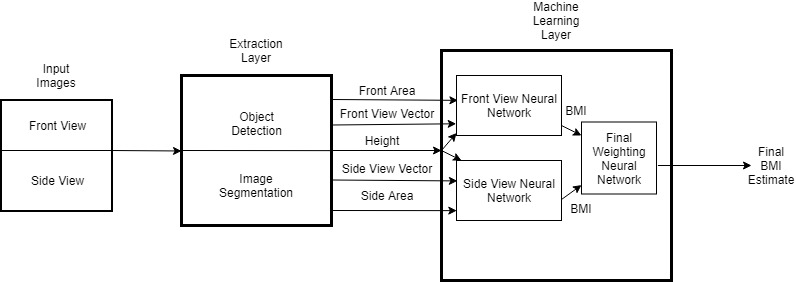
\includegraphics[width=\linewidth]{systemblock.jpg}
    \caption{System Block Diagram}
    \label{fig:systemblockdiagram}
\end{figure}
\end{landscape}
\begin{landscape}
\begin{figure}
    \centering
    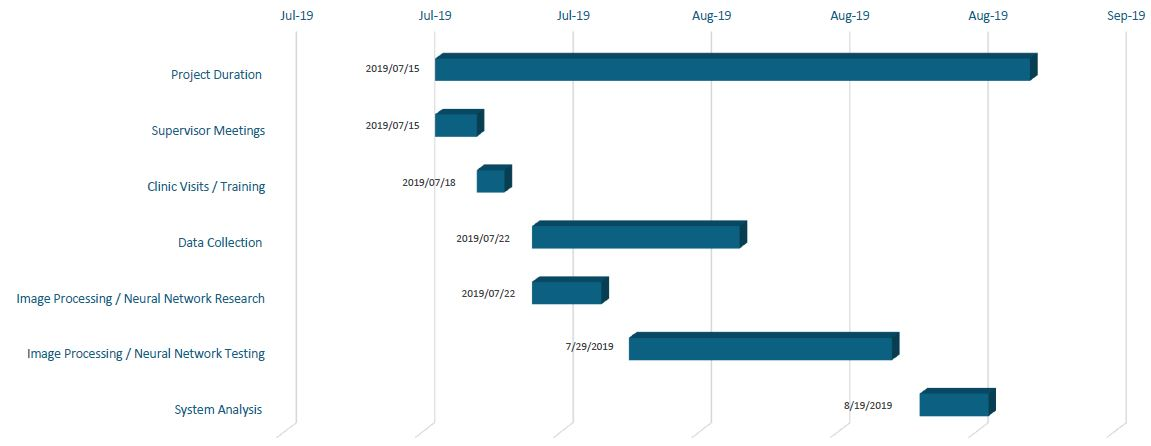
\includegraphics[width=\linewidth]{gannt.JPG}
    \caption{Gantt Chart showing project task breakdown and time allocation.}
    \label{fig:gantt}
\end{figure}
\end{landscape}